\section{Dressing Control}

The dressing problem, in its most abstract form, can be viewed as path planning with the goal of finding a path in the configuration space of the human such that the article of clothing ends up on the human's body in a desired manner. Unlike traditional path planning problems, the validity of the path depends on the evolution of another dynamic system, cloth. The need to consider the state of cloth invalidates many planning algorithms that utilize model predictive control, because the computational cost of cloth simulation is simply too high to be involved in any optimization loop. We remedy the issue based on two core ideas. First, we found that the state of cloth is extremely crucial, but only for a few brief moments in the entire path planning. We identify those ``cloth-sensitive'' actions and develop separate controllers for them. Second, for planning the cloth-sensitive moments, we exploit the geodesic information of cloth to make up for the lack of computation resources for online prediction.

We have designed a small set of primitive actions to control a character to put on a variety of garments using different styles. The two most important actions are \emph{alignment} and \emph{traversal}. We monitor the cloth state and solve an optimization at each time step only during the alignment phase. For other actions, we plan the entire path at the beginning of the action, and do not take the state of cloth into consideration.


% We have designed a small set of primitive actions to control a character to put on a variety of garments using different styles. The two most important actions are alignment and traversal. We found that while the feedback of the cloth state is crucial in alignment, feedback plays a less important role in other actions. For this reason, we monitor the cloth state and solve an optimization based on it at each time step only during the alignment phase. For other actions, we plan the entire path at the beginning of each action, which does not take the cloth state into consideration.

\subsection{Alignment}

The first step to putting on a garment is to align one body part, such as an end effector, with a cloth feature. For example, to align one hand with the armhole, or one foot with the waistband. In alignment, we typically choose a loop of vertices as the cloth feature and the goal is to control the end effector to pass through this loop. However, the target cloth feature is often folded and occluded by other parts of the cloth. It is not directly visible or reachable from the current end effector location. Furthermore, the alignment is a process of chasing a moving feature which has nonlinear dynamics and complex deformations. It is difficult to predict the movement of the feature without simulating the entire cloth, but the computation cost of cloth simulation makes this approach infeasible. Worse yet, as the end effector approaches the feature, it is highly likely that it will collide with the cloth in the neighborhood of the feature and knock the target away.  To address these challenges, we design a cloth-aware, feedback controller for the alignment action.

Our alignment controller first finds an intermediate goal towards the target feature, and then move the end effector a small distance towards this goal in a way that minimizes the chance to knock away the target feature. These two steps are performed iteratively until the end effector successfully reaches the feature. 

\ignorethis{
\begin{algorithm}[t]
  Align(skel, body, cloth, $\hat{\vc{q}}$)\\
  \Begin
    {
      \While{IsAligned(body, cloth.feature) $=$ False}
            {
              \tcc{Find the direction towards an intermediate goal.}
              \vc{R, t} $\leftarrow$ body.GetTransformation()\;
              camDirs[6] $\leftarrow$ \{$\pm\vc{R}$.Col(0), $\pm\vc{R}$.Col(1), $\pm\vc{R}$.Col(2)\}\;
              cubicMap $\leftarrow$ \{\}\;
              fov $\leftarrow$ $\pi / 2$\;
              asp $\leftarrow$ 1\;
              \ForEach{\vc{d} in camDir}
              {
                cam $\leftarrow$ SetCamera($\vc{t}$, $\vc{d}$, fov, asp)\;
                img $\leftarrow$ cam.Render(cloth.Mesh)\;
                cubicMap.Add(img)\;
              }
              imgIdx, u, v $\leftarrow$ cubicMap.BrightestPixel()\;
              $\vc{d}\leftarrow$ ComputeWorldDirFromCubicMap(imgIdx, u, v)\;

              \tcc{Move the end effector towards the intermediate goal.}
              $\hat{\vc{p}} \leftarrow \vc{t} + \alpha \vc{d}$\;
              opt $\leftarrow$ SetupIK($\hat{\vc{p}}$, $\hat{\vc{q}}$)        \tcp*{Equation \ref{eq:IK} and \ref{eq:collision}}
              opt.obj.Add($E_{orientation}$) \tcp*{Equation \ref{eq:orientation}}
              opt.con.Add($C_{speed}$) \tcp*{Equation \ref{eq:speed}}
              $\vc{q} \leftarrow$ opt.Solve()\;

              skel.SetPose($\vc{q}$)\;
              cloth.Simulate()\;
            }
    }
    \caption{Pseudocode of the alignment control.}
    \label{alg:alignment}
\end{algorithm}
}

\begin{figure}[!t]
  \centering
  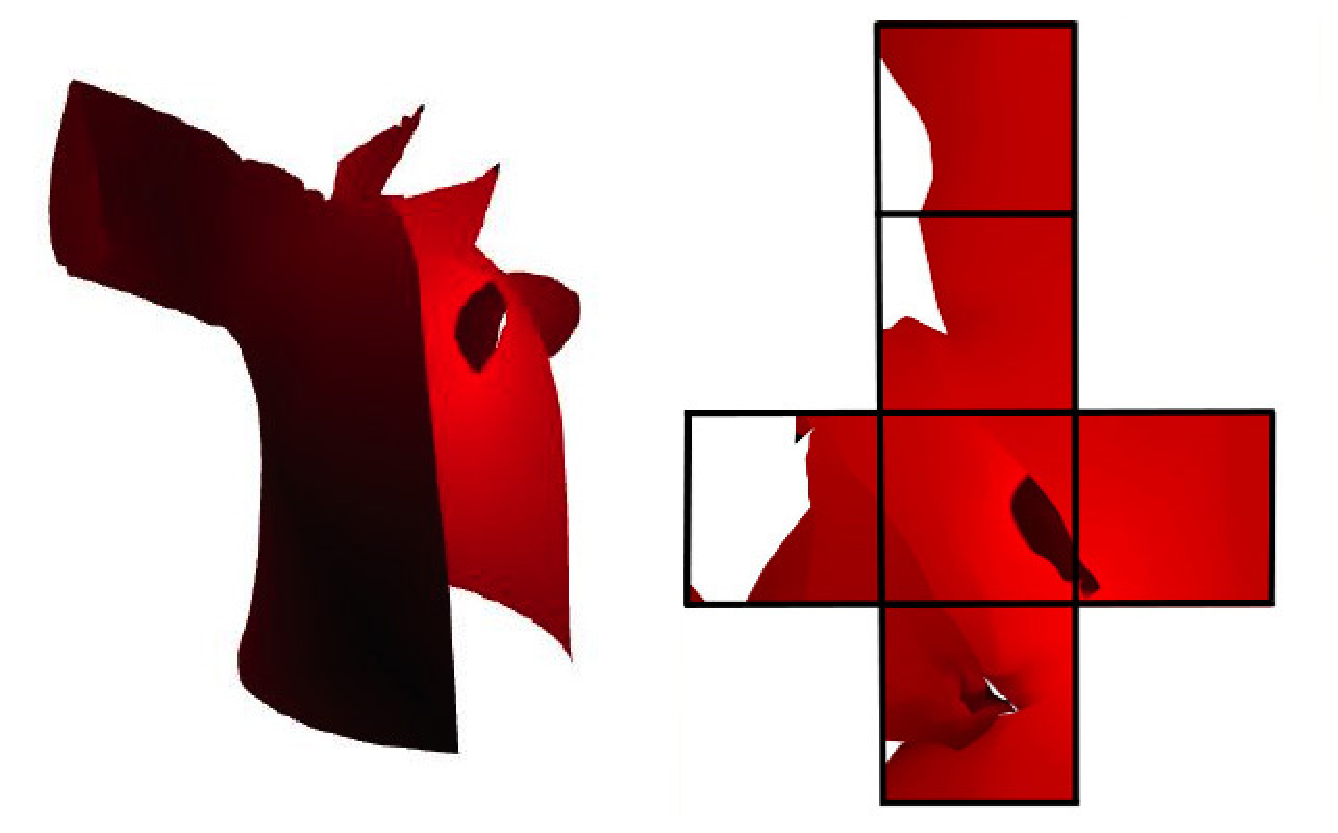
\includegraphics[width=2.6in]{images/geodesic}
  \caption{Left: The precomputed geodesic distance on the jacket to the left armhole. Brighter red means smaller distance. Right: A cubic map rendering of the geodesic distance when the character aligns his hand with the first sleeve (The first column of Figure~\ref{fig:jacket}).}
  \label{fig:geodesic}
\end{figure}


We set the intermediate goal as a point on the cloth which is visible from the end effector and has the smallest geodesic distance to the target feature. In our implementation, we find this point using rasterization techniques (Figure \ref{fig:geodesic} Right). We assign the color of vertices on the cloth mesh as their geodesic distances to the target. We place a camera at the end effector and render the cloth mesh into a cubic environmental map. The brightest pixel on the map corresponds to the direction to the intermediate goal. Note that we choose to render all six directions of the cubic map to allow the end effector to move not only forward, but also sideways and backward. Our experiments show that the ability to detect the intermediate goal behind the end effector drastically increases the success rate of the alignment. This is because a better intermediate goal might be behind the end effector and may only emerge when the end effector is sufficiently close to the current intermediate goal or when the end effector impacts the cloth, causing significant deformation. \karen{Verify the last sentence, please.} \alex{I edited the last sentence a little bit, but the presmise is correct.}

% , which is behind the end effector, might emerge as the it moves closer to the current intermediate goal or when it collides with the cloth. \karen{Because we sometimes overshoot the target?} \alex{Because we cannot assume that the best path into the cloth is a) in front of the camera or b) in the direction of the feature we are aiming for. This is especially true in the case of mocap or reference motion with places the end effector on the wrong side of the garment from the feature before alignment.} \jie{This is because a better position to aim at, which is behind the end effector, might emerge as the it moves closer to the current intermediate goal or when it collides with the cloth.}

However, the cloth geometry is represented as a single-layer triangular mesh, which means that there is no difference between a point at the outer and the inner surface of the cloth. Since the end effector needs to reach the target feature on a particular side of the cloth, we duplicate the mesh into two layers. These two layers are connected at their boundary. We precompute the geodesic distance on the two-layer cloth mesh using breadth first propagation starting from the feature vertices on the intended layer. For example, Figure \ref{fig:geodesic} visualizes the geodesic distance from the left armhole on the inner side of jacket. Note that the vertices inside the sleeve have large geodesic distances because we restrict the direction of initial distance propagation to the opposite side of the sleeve. Otherwise, the hand could align with the armhole by going through the cuff. 

To move the end effector towards the intermediate goal, we formulated an optimization to solve a collision-free inverse kinematics (IK) problem. The solution moves the character's end effectors to the desired locations, keeps the full body motion similar to the reference, and guarantees that the body parts do not overlap with each other.

\begin{align}
\label{eq:IK}
  \min_{\vc{q}} & ||\vc{q} - \hat{\vc{q}}||_\vc{w}^2 \\
  \nonumber  \mathrm{subject\;} \mathrm{to} & \\
  \nonumber  &\vc{p}(\vc{q}) = \hat{\vc{p}}\\
  \nonumber   &\vc{q}_{min} \leq \vc{q} \leq \vc{q}_{max}\\
  \nonumber   &||\vc{c}_i(\vc{q}) - \vc{c}_j(\vc{q})||_2^2 - (r_i + r_j)^2 \geq 0
\end{align}

where $\vc{q}$ are the joint angles, $\hat{\vc{q}}$ is the reference pose, $\vc{w}$ is a diagonal matrix that specifies the weight of each joint, $\vc{p}(\vc{q})$ are the end effector positions, $\hat{\vc{p}}$ are the target positions, $\vc{q}_{min}$ and $\vc{q}_{max}$ are the joint limits. The last constraint prevents inter-body penetrations. We approximate the collision volume of each body with multiple spheres and enforce no penetration for each pair of spheres that belong to different bodies. $\vc{c}_i$ and $r_i$ in the constraint are the center and radius of the $i$th sphere.

Given the direction to the goal $\vc{d}$ and the current end effector location $\vc{p}$, we set the desired end effector position $\hat{\vc{p}}$ at the next time step to be
\begin{equation}
  \hat{\vc{p}} = \vc{p}^n+\alpha\vc{d}
  \label{eq:target}
\end{equation}
where $\alpha$ is the user-specified step size. We choose the initial character pose when the alignment starts as the reference $\hat{\vc{q}}$ throughout the whole alignment phase. This reference pose has very little effect on the degrees of freedom active in the alignment task (\eg wrist, elbows), but stabilizes other degrees of freedom not involved in other constraints or objective terms in Equation \ref{eq:IK} (\eg knees in the jacket example).

In addition to the above IK formulation, we found that the orientation of the end effector also plays an important role in the alignment action. Since the end effector needs to weave through a tight and winding space between folds of the cloth, its orientation should be aligned with its direction of motion. This way of moving reduces the space swept by the end effector, lowering its chance to collide with the nearby cloth and minimizing the normal impacts if collisions happen. We add the following objective to the optimization to regulate the orientation of the end effector.

\begin{equation}
  E_{orientation} = 1-\vc{d}^T\vc{r(q})
  \label{eq:orientation}
\end{equation}
where $\vc{r(q)}$ is the direction from the center to the tip of the end effector.

We also limit the joint speed within a certain threshold to ensure the smoothness of the motion.
\begin{equation}
  -\dot{\vc{q}}_{max} \leq \frac{\vc{q} - \vc{q}^n}{\Delta t} \leq \dot{\vc{q}}_{max}
  \label{eq:speed}
\end{equation}
where $\vc{q}^n$ is the current pose, $\Delta t$ is the time step, and $\dot{\vc{q}}_{max}$ is the maximum allowed speed.

Finally, to determine whether the alignment action has succeeded, we first find a plane that best fits the cloth feature. We then project the feature vertices onto this plane. If the line segment linking the parent joint of the end effector to its center intersects the plane within the polygon formed by the projected feature, the alignment has succeeded and we move on to the next action in the queue.
%We then project both the center of the end effector and the vertex loop of the feature onto this plane. If the center of the end effector has passed over \karen{rephrase this. ``on the other side of''?} this plane and its projection is within the projected feature loop,


\subsection{Traversal}
After alignment, the center of the end effector has passed the desired cloth feature. However, at this point, the feature can still easily fall out of control due to gravity or inappropriate end effector motions. We design a traversal action to further secure the alignment and bring the feature to its final destination. Examples of traversal include stretching an arm into a sleeve until the feature reaches the shoulder or dragging the waistband of the pants up to the waist. We found that unlike alignment, the feedback from the state of cloth does not play an important role during traversal. We therefore design a feed-forward controller which plans the joint trajectory for the entire action at the beginning of the traversal. We first compute a series of desired targets of the end effector relative to the other limb. We then solve the collision-free IK (Equation~\ref{eq:IK}) for their corresponding full body poses, which are used as keyframes for the traversal motion. Although these keyframes are free of self collision among body parts, directly interpolating them can lead to inter-body penetrations. For this reason, we apply bi-directional Rapidly Expanding Random Tree (RRT) \cite{LaValleK:2001} to find a collision free trajectory between adjacent keyframes. RRT is a stochastic search method that finds collision-free paths in a given configuration space. In our case, the configuration is the set of joint positions for the relevant limbs.

We observed that in daily dressing activities, the traversal action can be categorized into two types. In the first type, the limb to be dressed remains relatively passive while another limb \emph{drags} the cloth along it. In the second type, the limb \emph{stretches} itself to pass through the tubular part of the cloth without assistance from other limbs. This situation is often seen when putting on the second sleeve of a jacket. To accomodate both types of traversal, we set up different objectives and constraints in the IK formulation.


\begin{figure*}[!t]
  \centering
  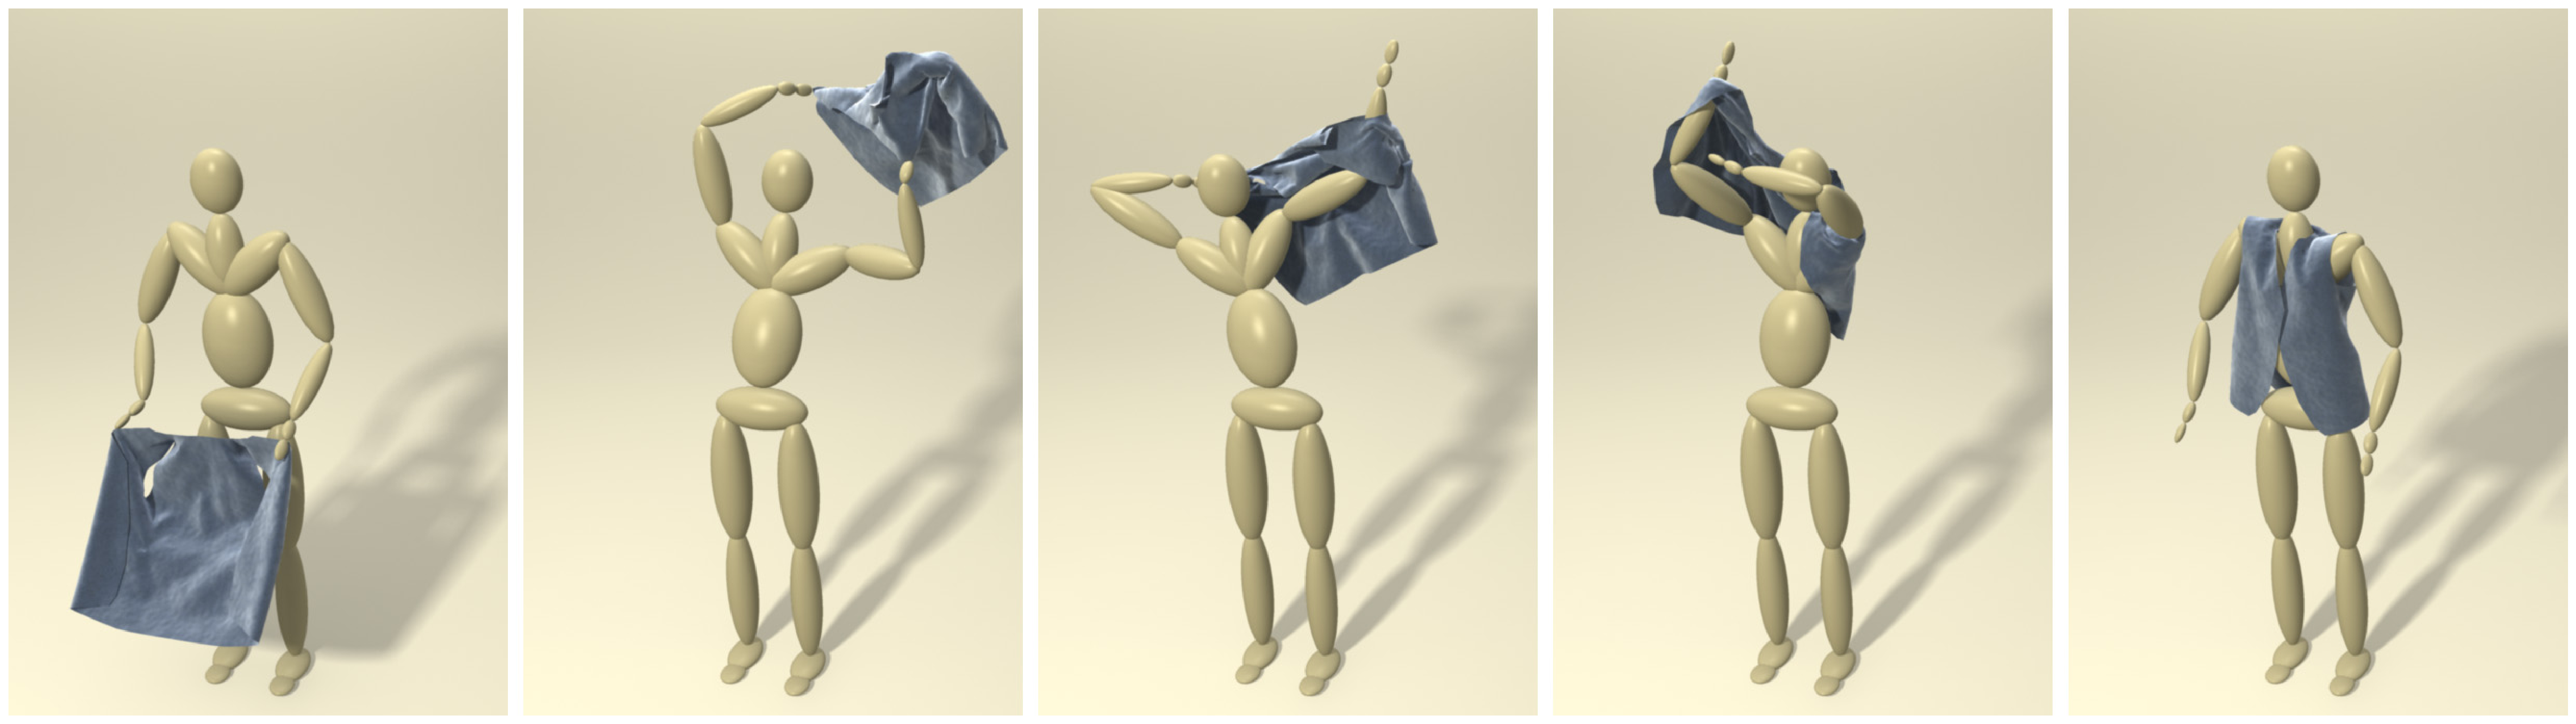
\includegraphics[width=\textwidth]{images/vest}
  \caption{A character puts on a vest by swinging it around his neck.}
  \label{fig:vest}
\end{figure*}

\begin{figure*}[!t]
  \centering
  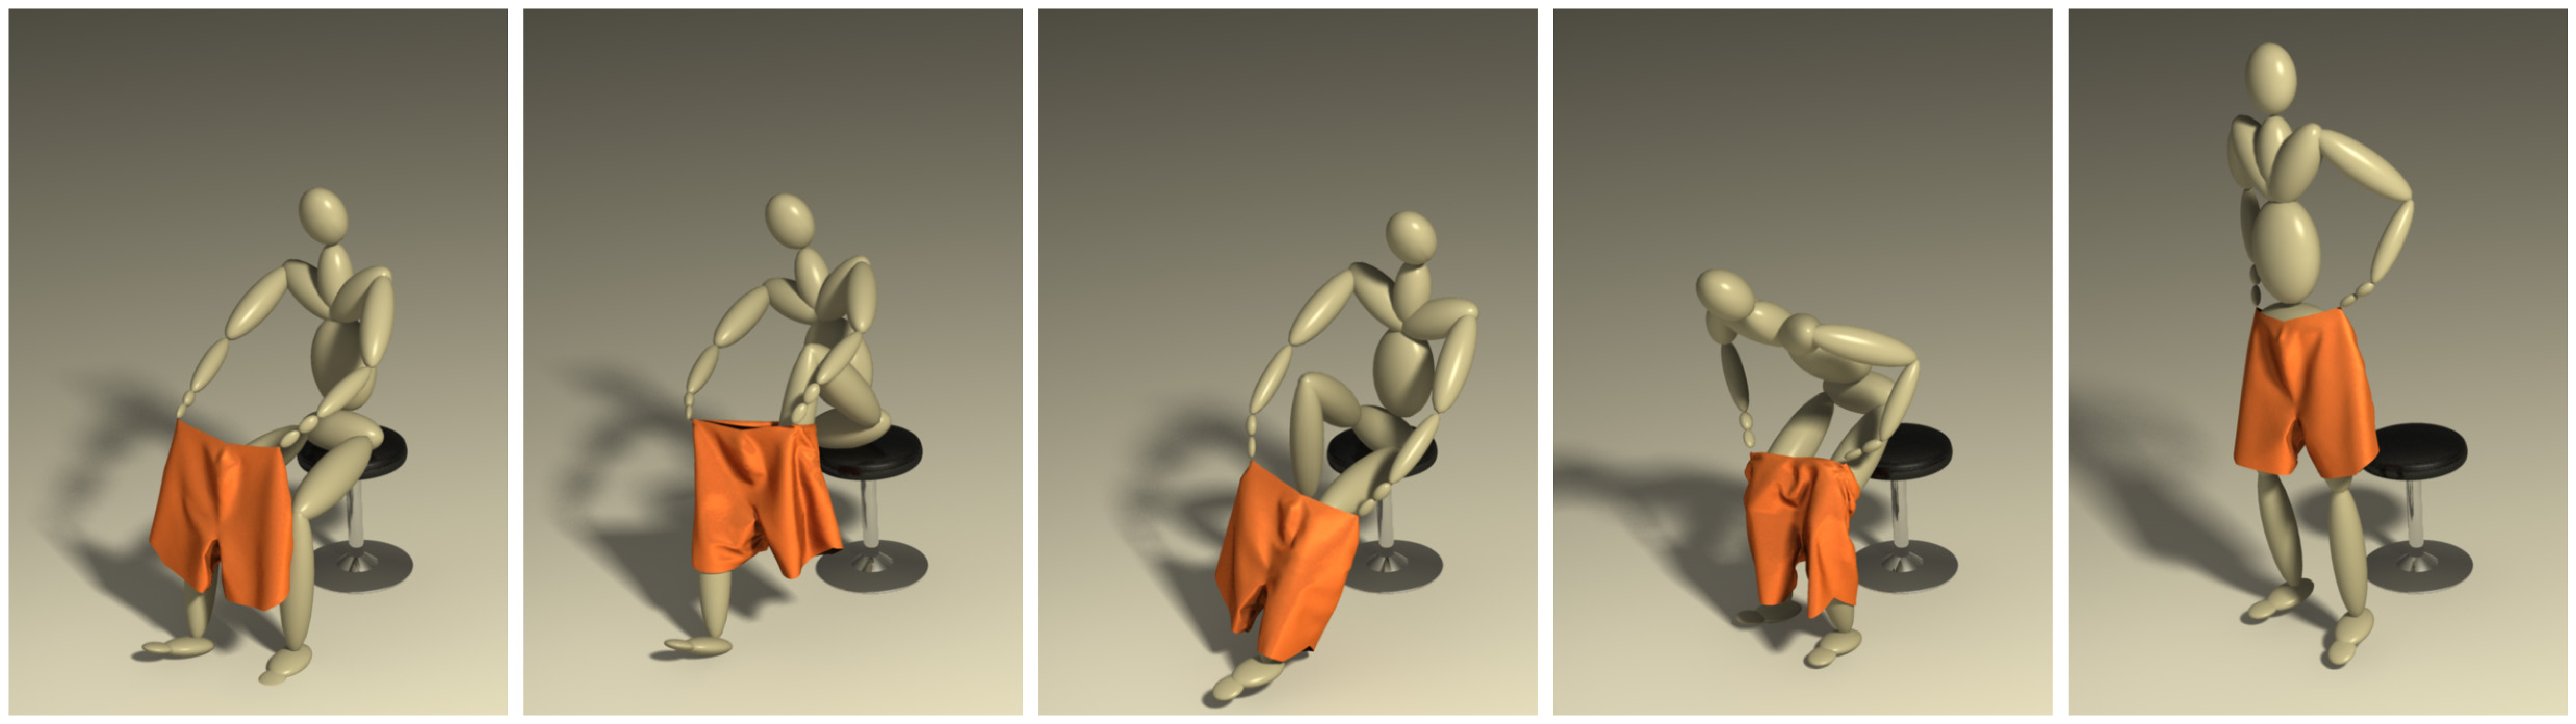
\includegraphics[width=\textwidth]{images/shortsSitting}
  \caption{A character puts on a pair of shorts in a sitting pose.}
  \label{fig:shorts1}
\end{figure*}



\paragraph{Dragging.} In the first case, a user can specify one end effector to drag the cloth and a set of body parts $\{B_1 ,..., B_n\}$ that the cloth should be dragged upon. We use the positions of the parent joints of those bodies as path nodes. For example, if the character is using his or her right hand to dress the left arm, the path nodes are the left wrist, the left elbow and the left shoulder. For each of the path node $\vc{p}_i$, we set the target end effector location $\hat{\vc{p}}=\vc{p}_i$ in Equation~\ref{eq:IK}, and solve the collision-free IK for one keyframe of the dragging motion.

\paragraph{Stretching.} \karen{I made some change sin this paragraph. Please verify.}In the second case of traversal, one limb straightens into the cloth tube without assistance from other end effectors. The most frequent failure in this task is that the cloth moves together with the stretching limb, preventing the feature from moving along the limb toward its destination. An effective strategy humans frequently utilize is to use another body part as an anchor to keep the cloth from moving with the stretching limb. We call this body part an \emph{anchor node}. For example, when stretching the right arm into a sleeve as shown in the third column of Figure \ref{fig:jacket}, the anchor node is the left shoulder. Without anchoring the shoulder, the stretching action could fail easily because the IK solver might yield a pose in which the shoulder moves along with the stretching arm, resulting in very little relative movement between the arm and the sleeve. We implemented the anchor node as an additional constraint in the optimization (Equation~\ref{eq:IK}).

\begin{align}
  \label{eq:fixtureNode}
  \nonumber  \vc{p}(\vc{q})& = \vc{p}^n
\end{align}
where $\vc{p}^n$ and $\vc{p(q)}$ are the center of the fixture node at the current and the next time step.

Besides the anchor node, a correct stretching direction is also critical. We use the direction from the center of the anchor node to the current end effector location as the stretching direction. Along this direction, the friction force caused by the stretching limb is canceled by the tension for of the cloth pulling from the anchor node. This prevents the cloth feature from moving with the end effector so that the limb can further pass through the feature. We add an objective term to Equation \ref{eq:IK} to specify the desired stretching direction.
\begin{equation}
  E_{stretch} = \sum_i1 - \vc{d}_{stretch}^T\vc{r_i(q)}
  \label{eq:stretching}
\end{equation}
where $\vc{d}_{stretch}$ is the desired stretching direction and $\vc{r_i(q)}$ is the longest principal axis of the $i$th body of the limb. \karen{All directions are normalized, right?}\alex{yes}

Together with the stretching direction objective (Equation~\ref{eq:stretching}) and the anchor node constraint (Equation~\ref{eq:fixtureNode}), the collision-free IK (Equation~\ref{eq:IK}) solves for the keyframe pose at the end of the stretching action (the fourth column of Figure~\ref{fig:jacket}).

\subsection{Other Actions}

\paragraph{Tracking.} To preserve the dressing style specified by the user, we used the tracking action to follow the reference motion $\hat{\vc{q}}(t)$. In most cases, it simply uses the next pose in the reference motion.
\begin{displaymath}
\vc{q} = \hat{\vc{q}}^{n+1}
\end{displaymath}
However, after alignment and traversal, the joint trajectory of the character could deviate from the reference motion. Interpolation from the current pose to a pose in the reference motion is necessary for a smooth animation. To prevent inter-body collisions during the interpolation, similar to the traversal action, we apply RRT for a collision free path and follow this path to the target pose.


\paragraph{Grip and release.}
The grip action models the grasping of the character's hand. The cloth feature moves together with the character's hand if it is gripped. This action constrains the vertices in the cloth feature to the local frame of the end effector.
\begin{displaymath}
\vc{p}_w = \vc{Rp} + \vc{t}
\end{displaymath}
where $\vc{p}_w$ is the world position of a vertex in the cloth feature, $\vc{p}$ is the local position of this vertex in the end effector's frame, $\vc{R}$ and $\vc{t}$ are the rotation and translation of the end effector. The release action simply removes the above constraints so that the cloth feature no longer moves with the end effector.

\paragraph{Idling.} This action freezes the character's motion for a user-specified time period. The main purpose of this action is to wait the clothes to settle before proceeding to the next dressing action.